\documentclass[11pt,a4paper]{article}
\usepackage[spanish,es-nodecimaldot]{babel}	% Utilizar español
\usepackage[utf8]{inputenc}					% Caracteres UTF-8
\usepackage{graphicx}						% Imagenes
\usepackage[hidelinks]{hyperref}			% Poner enlaces sin marcarlos en rojo
\usepackage{fancyhdr}						% Modificar encabezados y pies de pagina
\usepackage{float}							% Insertar figuras
\usepackage[textwidth=390pt]{geometry}		% Anchura de la pagina
\usepackage[nottoc]{tocbibind}				% Referencias (no incluir num pagina indice en Indice)
\usepackage{enumitem}						% Permitir enumerate con distintos simbolos
\usepackage[T1]{fontenc}					% Usar textsc en sections
\usepackage{amsmath}						% Símbolos matemáticos
\usepackage{listings}
\usepackage{algorithm}
\lstdefinelanguage{PDDL}
{
  sensitive=false,    % not case-sensitive
  morecomment=[l]{;}, % line comment
  alsoletter={:,-},   % consider extra characters
  morekeywords={
    define,domain,problem,not,and,or,when,forall,exists,either,
    :domain,:requirements,:types,:objects,:constants,
    :predicates,:action,:parameters,:precondition,:effect,
    :fluents,:primary-effect,:side-effect,:init,:goal,
    :strips,:adl,:equality,:typing,:conditional-effects,
    :negative-preconditions,:disjunctive-preconditions,
    :existential-preconditions,:universal-preconditions,:quantified-preconditions,
    :functions,assign,increase,decrease,scale-up,scale-down,
    :metric,minimize,maximize,
    :durative-actions,:duration-inequalities,:continuous-effects,
    :durative-action,:duration,:condition
  }
}
\lstdefinelanguage{JSHOP}
{
  sensitive=false,    % not case-sensitive
  morecomment=[l]{;}, % line comment
  alsoletter={:,-},   % consider extra characters
  morekeywords={
    defdomain,defproblem,not,and,or,imply,forall,assign,call,nil,
    :first,:sort-by,:immediate,:unordered,:operator,:method,:protection,:-
  }
}

% Comando para poner el nombre de la asignatura
\newcommand{\asignatura}{Técnicas de los Sistemas Inteligentes}
\newcommand{\autor}{Vladislav Nikolov Vasilev}

% Configuracion de encabezados y pies de pagina
\pagestyle{fancy}
\lhead{\autor{}}
\rhead{\asignatura{}}
\lfoot{Grado en Ingeniería Informática}
\cfoot{}
\rfoot{\thepage}
\renewcommand{\headrulewidth}{0.4pt}		% Linea cabeza de pagina
\renewcommand{\footrulewidth}{0.4pt}		% Linea pie de pagina

\begin{document}
\pagenumbering{gobble}

% Pagina de titulo
\begin{titlepage}

\begin{minipage}{\textwidth}

\centering

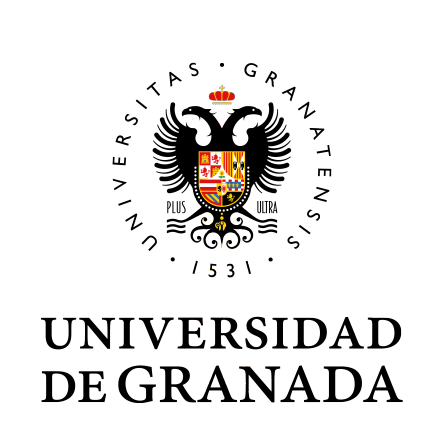
\includegraphics[scale=0.5]{img/ugr.png}\\

\textsc{\Large \asignatura{}\\[0.2cm]}
\textsc{GRADO EN INGENIERÍA INFORMÁTICA}\\[1cm]

\noindent\rule[-1ex]{\textwidth}{1pt}\\[1.5ex]
\textsc{{\Huge PRÁCTICA 2\\[0.5ex]}}
\textsc{{\Large Planificación Clásica\\}}
\noindent\rule[-1ex]{\textwidth}{2pt}\\[3.5ex]

\end{minipage}

\vspace{0.5cm}

\begin{minipage}{\textwidth}

\centering

\textbf{Autor}\\ {\autor{}}\\[2.5ex]
\textbf{Rama}\\ {Computación y Sistemas Inteligentes}\\[2.5ex]
\vspace{0.3cm}


\includegraphics[scale=0.3]{img/etsiit.jpeg}

\vspace{0.7cm}
\textsc{Escuela Técnica Superior de Ingenierías Informática y de Telecomunicación}\\
\vspace{1cm}
\textsc{Curso 2018-2019}
\end{minipage}
\end{titlepage}

\pagenumbering{arabic}
\tableofcontents
\thispagestyle{empty}				% No usar estilo en la pagina de indice

\newpage

\setlength{\parskip}{1em}

\section{Ejercicio 1}

A continuación se ofrece una descripción de las decisiones de diseño tomadas a la hora de realizar el ejercicio 1.

\subsection{Ejercicio 1.a}

Para representar los objetos del mundo se han utilizado tipos, y para dar un mayor nivel de abstracción, se han utilizado supertipos.
Por ejemplo, los distintos tipos de objetos (Manzana, Algoritmo, etc.) se han englobado bajo el supertipo \textit{items} para
poder facilitar referirse a cualquiera de ellos. Lo mismo pasa con los personajes, los cuáles han sido englobados bajo el supertipo
\textit{npc} para referirse a cualquiera de ellos. Y para todos los objetos que pueden ser puestos en alguna posición (jugador,
personaje al que dar un objeto y objeto) se han englobado bajo el supertipo \textit{locatable}. Todo esto se ha hecho, tal y como
se ha mencionado hace un momento, con el objetivo de facilitar la generalización al poder referirnos posteriormente a cualquier tipo
de personaje u objeto mediante un supertipo, en vez de tener que indicar el tipo concreto de un objeto.

A continuación se puede ver el dominio:

\begin{algorithm}[H]
\begin{lstlisting}[
  caption={Representación del dominio.},
  label={lst:pddlmove},
  language=PDDL]
(:types items npc Player - locatable
  	Oscar Manzana Algoritmo Oro Rosa - items
  	Princesa Principe Bruja Profesor Leonardo - npc
  	Player
  	zone
)
\end{lstlisting}
\end{algorithm}

\subsection{Ejercicio 1.b}

En este apartado se han representado los predicados básicos del dominio. Para representar las orientaciones del personaje y 
las posiciones relativas de dos zonas adyacentes (conexas), se han utilizado constantes que hacen referencia a cada uno de los
cuatro puntos cardinales (norte, sur, este y oeste). Se han elegido constantes debido a que son valores que no se van a instanciar
(no se van a crear variables de éstos ya que no tiene mucho sentido tenerlas), y como tal representan más un atributo o una propiedad
que un concepto u objeto.

En cuanto a los predicados, se han definido predicados para la orientación del jugador, las conexiones de zonas, las posiciones de
objetos, personajes y jugador (objetos con posición) y algunos predicados más que comentaremos.

Para la orientación del jugador, se utiliza el predicado \textbf{oriented}, el cuál indica qué jugador tiene qué orientación. Para
la localización de un objeto con posición se ha utilizado el predicado \textbf{at} que indica que el objeto con posición se encuentra
en una determinada zona. Se puede ver que aquí se ha utilizado una abstracción sobre un conjunto de conceptos para facilitar la
representación (como se indicó en el apartado anterior). Para representar las conexiones entre zonas se utiliza el predicado
\textbf{connected}, el cuál especifica que la primera zona está conectada zon la segunda zona mediante un punto cardinal (el cuál
reutiliza las constantes de orientación). Por ejemplo, si tuviésemos que desde una zona \textit{z1} se puede llegar a una zona
\textit{z2} la cuál se sitúa en el sur, tendríamos \textbf{(connected z1 S z2)}. Esto se ha hecho así para facilitar más adelante la
acción del giro, para poder comprobar más fácil si la orientación del jugador coincide con la de la zona a la que se quiere ir. El
predicado \textbf{emptyhand} indica que un determinado jugador tiene la mano vacía, y por tanto puede coger un objeto. Es importante
indicar esto, ya que si no, no habría forma de controlar si un jugador no tiene ya un objeto en la mano (recordemos que de momento
solo puede llevar un objeto). El predicado \textbf{taken} representa que un objeto (tipo \textit{item}) ha sido cogido por un jugador
determinado. El predicado \textbf{given} indica que un determinado objeto ha sido entregado a cualquier personaje. Esto se hace con el
objetivo de que el jugador no pueda quitarles a los personajes aquellos objetos que les hayan sido entregados. A parte de estos
predicados básicos, se tiene una función numérica \textbf{received} que indica cuántos objetos ha recibido un determinado personaje.
Cada vez que recibe uno, se incrementa el valor. Esto se ha hecho así para tener una especie de contador de objetos recibidos, el cuál
nos será útil más adelante. A continuación se pueden ver los predicados representados:

\begin{algorithm}[H]
\begin{lstlisting}[
  caption={Representación de predicados básicos.},
  label={lst:pddlmove},
  language=PDDL]
(:constants N S E W - orientation)
(:predicates
	(oriented ?p - Player ?o - orientation)
  	(at ?l - locatable ?z - zone)
  	(connected ?z1 - zone ?o - orientation ?z2 - zone)
  	(emptyhand ?p - Player)
  	(taken ?obj - items ?p - Player)
  	(given ?obj - items)
)
(:functions
  	(received ?n - npc)
)
\end{lstlisting}
\end{algorithm}

\subsection{Ejercicio 1.c}

Para este apartado se han creado acciones para girar al jugador tanto a la derecha como a la izquierda, desplazarse de una
zona a otra e interactuar con objetos y personajes.

Debido a que el código de las acciones es muy extenso, no se va a adjuntar en la memoria, si no que se va a comentar su funcionamiento
a algo nivel:

\begin{itemize}
	\item Para las acciones de giro, se comprueba la orientación del personaje, y según esta orientación se le asigna una nueva
	dependiendo del tipo de giro. Antes de esto, obviamente, se elimina la orientación antigua.
	\item Para moverse de una zona \textit{z1} a una zona \textit{z2}, se tiene que dar que el jugador se encuentre en la zona
	\textit{z1}, que las dos zonas estén conectadas y que el jugador esté orientado correctamente, ya que si no, tendrá que girar
	antes para orientarse correctamente. Al aplicar la acción, se cambia la posición del jugador y se elimina la anterior.
	\item Para coger un objeto se tiene que dar que el jugador tenga la mano vacía, ya que el jugador no puede coger más de un
	objeto simultáneamente (tendría que dejar el otro). Una vez que se aplica el objeto, el jugador deja de tener la mano vacía,
	el objeto no está en la zona en la que se encontraba y se indica que el objeto ha sido cogido por un determinado jugador.
	\item Para dejar un objeto, se tiene que dar que el jugador tenga cogido el objeto. Al dejarlo, se indica que el jugador ya no
	tiene cogido el objeto, que tiene la mano vacía y que el objeto se encuentra en la zona donde se encuentra actualmente el jugador.
	\item Para entregar un objeto, el jugador tiene que encontrarse en la misma zona que el personaje y tiene que tener cogido un
	objeto. Cuando se lo da, se indica que el jugador ya no tiene el objeto y que vuelve a tener la mano vacía. También se indica
	que el objeto se encuentra en la zona del personaje para intentar seguir una coherencia con la descripción del mundo, ya que
	al ser entregado no ``desaparece'', si no que el objeto se encuentra en una determinada zona del espacio, solo que ahora en
	posesión de un personaje. Para que no pueda volver a ser cogido y para representar que un personaje tiene posesión del objeto, se
	indica que el objeto ha sido entregado a un determinado personaje, y se incrementa el número de objetos que ha recibido dicho
	personaje. Ésto último, como se ha comentado antes, será muy significativo posteriormente.
\end{itemize}

\subsection{Ejercicio 1.d}

En este ejercicio se han planteado 2 problemas. El primero es un problema con 25 zonas con la forma de una matriz $5 \times 5$, donde
cada zona está conectada con sus zonas adyacentes. Se han situado 5 personajes en el mapa (uno de cada clase) y 5 objetos (uno de cada
tipo), de tal forma que estuviesen más o menos dispersos de igual forma. Se ha situado al jugador en el centro del mapa y orientado
hacia el sur (como en todos los problemas, ya que no se especifica nunca que el jugador tenga una determinada orientación inicial).
El objetivo era que cada personaje tuviese al menos un objeto. Para representar este objetivo sin decir explícitamente qué jugador
debe tener qué objeto, aquí ha venido muy bien el contador \textbf{received} del que se habló anteriormente, ya que simplemente
bastaba con indicar que cada personaje tenía que recibir una cantidad de objetos mayor o igual que 1. Con esto, se han creado 2
planes: uno sin optimizar y uno optimizando. El resultado que se ha obtenido es que las dos planificaciones han obtenido el mismo
plan, con lo cuál en este caso, la optimización no ha sido un factor muy importante.

Se ha planteado un segundo problema con 12 zonas y de nuevo 5 objetos y 5 personajes, cada uno de una clase. El objetivo ha sido, de
nuevo, que cada personaje tuviese un objeto, pero además de eso, que el jugador estuviese en la zona 3 y orientado al norte. En este
caso se han obtenido de nuevo dos planes: uno sin optimización y uno optimizando. En este caso, el plan sin optimización es más largo
que el que se ha obtenido optimizando con \textit{BFS}, con lo cuál aquí si que influye la optimización, posiblemente debido a las
conexiones de las zonas y a las distribuiciones de los personajes y objetos.

\section{Ejercicio 2}

A continuación se ofrece una descripción de las decisiones de diseño tomadas a la hora de realizar el ejercicio 2.

\subsection{Ejercicio 2.a}

Para considerar las distancias, se han añadido dos nuevas funciones a las que ya teníamos antes. La primera es la función
\textbf{distance}, que indica el coste del camino que une una zona con la otra. La segunda es \textbf{traveled}, que indica
cuánta distancia ha recorrido un determinado jugador, en caso de que haya más de uno. Se han utilizado funciones debido a que
son lo único que nos permite trabajar con valores numéricos en PDDL. A continuación se pueden ver las nuevas funciones:

\begin{algorithm}[H]
\begin{lstlisting}[
  caption={Representación de las funciones de coste y distancia viajada.},
  label={lst:pddlmove},
  language=PDDL]
(:functions
    (distance ?z1 ?z2 - zone)
    (traveled ?p - Player)
)
\end{lstlisting}
\end{algorithm}

Adicionalmente se ha modificado la acción \textbf{move}, para que cuando un jugador se mueva de una zona a otra se incremente el
valor de \textbf{traveled} de dicho jugador con el valor de \textbf{distance} correspondiente.

\subsection{Ejercicio 2.b}

En este ejercicio se han planteado de nuevo dos problemas. El primero de ellos tiene exactamente la misma descripción que el problema
de las 25 zonas del ejercicio anterior, solo que se han añadido costes entre las zonas. El plan que se obtuvo del planificador sin
era el más largo, pero a la vez también el más rápido, ya que no buscaba minimizar la distancia total viajada. Se ha probado también a
obtener un plan con optimización por \textit{BFS} y por búsqueda con $g = 1$ y $h = 1$. Los resultados es que en el primer caso se
obtuvo un plan más corto que el original con un coste de 46. En el segundo caso se obtuvo un plan aún más corto que el caso anterior
con un coste de 34, pero se ha tardado mucho en obtener el plan. Por tanto, podemos concluir que la búsqueda con $g = 1$ y $h = 1$ es
la que más tarda en obtener un resultado, pero que siempre obtiene el camino de coste óptimo, y que el peso que se le asigna a la
heurística es importante, ya que en el primer caso hace más una búsqueda heurística mientras que en el segundo caso hace una búsqueda
más equilibrada.

El segundo problema sigue la misma descripción que el problema de las 12 zonas del ejercicio anterior, solo que se han añadido costes.
El plan que se ha obtenido sin optimizar es el más corto, pero no tiene en cuenta las distancias. El que se ha obtenido por
\textit{BFS} es una acción más largo que el anterior, pero obtiene el camino óptimo (a diferencia del caso anterior). La búsqueda
equilibrada obtiene un plan con el mismo coste pero con 2 acciones más que el anterior, además de que tarda más tiempo en obtenerlo.

\section{Ejercicio 3}

A continuación se ofrece una descripción de las decisiones de diseño tomadas a la hora de realizar el ejercicio 3.

\subsection{Ejercicio 3.a}

En este ejercicio se han añadido una serie de nuevas constantes, tipos y predicados. Las constantes que se han añadido son para
representar el tipo de superficie de cada zona. Se han hecho contantes ya que no interesa tener instancias de ellas debido a que son
más una propiedad o atributo de un concepto que una entidad como tal.

Los tipos nuevos representan los dos nuevos tipos de objetos: la zapatilla y el bikini. Estos dos nuevos tipos han sido
englobados por el supertipo \textit{items}, ya que así es más fácil referirse a un objeto en general a la hora de cogerlo y/o dejarlo.

Los nuevos predicados permiten relacionar una zona con el tipo de superfície (esto es importante, ya que se tiene que comprobar qué
superfície tiene la zona a la que se va a mover el jugador para saber si puede ir por ahí o no) y si un objeto es una zapatilla o
un bikini, para saber si ese objeto se puede entregar o no a un personaje (no tiene sentido entregar estos objetos ya que sin ellos
el jugador pierde capacidad para desplazarse), lo cuál se comprobará en las acciones correspondientes.

Lo dicho anteriormente se puede ver a continuación:

\begin{algorithm}[H]
\begin{lstlisting}[
  caption={Modificación del dominio para permitir superfícies y nuevos objetos para el movimiento.},
  label={lst:pddlmove},
  language=PDDL]
(:types
 Oscar Manzana Algoritmo Oro Rosa Zapatilla Bikini - items
)
(:constants
	Bosque Agua Precipicio Arena Piedra - surface
)
(:predicates
	(terrain ?z - zone ?s - surface)
	(is_zapatilla ?o - items)
	(is_bikini ?o - items)
)
\end{lstlisting}
\end{algorithm}

En cuanto a las acciones, a la acción de entregar un objeto a un personaje se han añadido las precondiciones de que el objeto
no tiene que ser ni una zapatilla ni un bikini (lo cuál tiene sentido por lo que se ha comentado anteriormente, además de que
el hecho de tener esos dos predicados hace que sea más fácil saber si un objeto se puede entregar o no). A la acción de moverse
se le pasa como parámetro también un objeto y se comprueba si a la hora de desplazarse necesita ese objeto o no (por ejemplo, si
necesita ir a una zona de Bosque se comprueba si tiene un objeto de tipo zapatilla cogido). También se comprueba que la zona a la
que va a desplazarse no es un precipicio, ya que el jugador no puede desplazarse por ese tipo de superfícies.

\subsection{Ejercicio 3.b}

En este apartado se ha añadido la posibilidad de que el jugador lleve una mochila. Esto se ha representado con dos nuevos predicados:
uno que representa que un jugador determinado tiene la mochila vacía, y que por tanto puede insertar objetos dentro; y otro predicado
que indica que un jugador determinado tiene un objeto en su mochila (y que por tanto no está vacía). Se ha decidido hacer esto para
emular una especie de segunda mano con los predicados, ya que si hay múltiples jugadores, cada uno de ellos tiene una mochila
individuale en la que pueden meter un objeto como máximo, con lo cuál no tiene sentido que haya predicados referentes a la mochila
de manera global, si no específica para cada jugador (tal y como se hacía con la mano). A continuación se pueden ver estos nuevos
predicados:

\begin{algorithm}[H]
\begin{lstlisting}[
  caption={Modificación del dominio para permitir el uso de mochilas a los jugadores.},
  label={lst:pddlmove},
  language=PDDL]
(:predicates
	(emptybag ?p - Player)
	(inbag ?o - items ?p - Player)
)
\end{lstlisting}
\end{algorithm}

Respecto al apartado anterior, hace falta modificar algunas acciones de nuevo y añadir algunas nuevas. Se han añadido acciones para
meter y sacar un objeto de la mochila. En el primer caso, el jugador tiene que tener la mochila vacía y el objeto en la mano, y pasa
a tener el objeto en la mochila y la mano vacía. En el segundo caso, tiene que tener la mano vacía y un objeto en la mochila, y pasa
a tener el objeto en la mano y la mochila vacía. A la hora de mover un jugador, se comprueba también si tiene el objeto en la mochila.
A la hora de soltar un objeto, se comprueba antes si tiene espacio en la mochila, ya que no tiene mucho sentido soltar un objeto
y coger otro cuando el personaje tiene la mochila vacía.

\subsection{Ejercicio 3.c}

De nuevo se han probado dos problemas. El primero es el problema de las 25 zonas del ejercicio anterior, añadiendo ahora
superfícies que obliguen al jugador a plantearse si necesita coger un objeto que le permita desplazarse, además de un bikini y una
zapatilla, los cuáles se usarán para desplazarse. El planificador encontró un plan en muy poco tiempo sin dar ningún item que no
tocaba a ningún personaje. Se ha intentado optimizar el problema, pero debido al tamaño de este se obtenía una violación de segmento,
con lo cuál a partir de aquí se dejará de intentar optimizar este problema.

El segundo problema es una modificación del de 12 zonas de antes añadiendo una nueva zona que es un precipicio. Como en el caso
anterior, se han añadido superfícies y los nuevos objetos. El planificador encontró un plan tanto sin optimizar como con los dos
tipos de optimizaciones en un tiempo muy pequeño. Pero, a medida que se iba optimizando la distancia recorrida, el tamaño del plan
iba aumentando. De hecho, entre los dos planes optimizados, a pesar de tener el mismo coste, hay más acciones en el plan con la
heurística equilibrada que con la de \textit{BFS}.

\section{Ejercicio 4}

A continuación se ofrece una descripción de las decisiones de diseño tomadas a la hora de realizar el ejercicio 4.

\section{Ejercicio 5}

A continuación se ofrece una descripción de las decisiones de diseño tomadas a la hora de realizar el ejercicio 5.

\section{Ejercicio 6}

A continuación se ofrece una descripción de las decisiones de diseño tomadas a la hora de realizar el ejercicio 6.

\section{Ejercicio 7}

A continuación se ofrece una descripción de las decisiones de diseño tomadas a la hora de realizar el ejercicio 7.

\end{document}

